\documentclass[12pt]{extarticle}
\usepackage{manualdoprofessor}
\usepackage{fichatecnica}
\usepackage{lipsum,media9,graficos}
\usepackage[justification=raggedright]{caption}
\usepackage[one]{bncc}
\usepackage[squarebr]{gmverse}
\usepackage[acorde]{../edlab}


\begin{document}


\newcommand{\AutorLivro}{Charles Baudelaire}
\newcommand{\TituloLivro}{Pequenos poemas em prosa}
\newcommand{\Tema}{Ficção, mistério e fantasia}
\newcommand{\Genero}{Poema}
\newcommand{\imagemCapa}{./images/PNLD0010-01.png}
\newcommand{\issnppub}{978-65-994412-1-9}
%\newcommand{\issnepub}{---}
% \newcommand{\fichacatalografica}{PNLD0010-00.png}
\newcommand{\colaborador}{Bruno Gradella\\ e Vicente Castro}


\title{\TituloLivro}
\author{\AutorLivro}
\def\authornotes{\colaborador}

\date{}
\maketitle


\begin{abstract}\addcontentsline{toc}{section}{Carta ao professor}

\textbf{Charles Baudelaire} (Paris, 1821--\textit{id.}, 1867), escritor francês, é
 ainda hoje reverenciado como um dos paradigmas máximos da criação poética.
 Dono de uma imagética pujante e original, Baudelaire foi também um
 influente crítico de arte e um tradutor de grande envergadura. Alma
 inquieta e conturbada, antípoda de Goethe, segundo o famoso elogio de
 T. S. Eliot, Baudelaire via com desconfiança a era do progresso,
 entrevendo na modernidade uma morbidez oculta que sua sensibilidade
 extremada não tolerava. Em 1857, a publicação de \textit{As flores do mal}, sua
 obra-prima, ofende a moral burguesa e lhe vale um processo no qual é
 obrigado a pagar uma multa considerável, além de suprimir sete poemas do livro.
 Alguns dos sonetos ali encerrados
 já prefiguravam o simbolismo e o decadentismo, correntes que começavam a
 tomar corpo. Em \textit{Os paraísos artificiais} (1860), explora o potencial
 criador sob o efeito do ópio e do haxixe. Como tradutor, verte
 muitos dos contos e ensaios de  Edgar Allan Poe para o francês, tendo influído assim decisivamente
 para o futuro reconhecimento desse autor, que 
 exerceu influência em sua obra também. Solitário, doente e sem recursos,
 morre em 1867.

\textbf{Pequenos poemas em prosa}, obra póstuma, publicada em 1869 na reunião
 de escritos do autor feita por Théodore de Banville e Charles Asselineau,
 consumiu mais de dez anos até sua feição definitiva, em 1866. Muitos dos poemas
 já haviam aparecido em jornais e receberam de pronto a estima e a
 admiração da crítica e do público. Figura, em importância, ao lado de
 \textit{As flores do mal} na obra de Baudelaire e ombreia com
 as mais importantes páginas já escritas da literatura universal. Esta edição
saiu à luz pela primeira vez em 1988 pela editora da Universidade de Santa Catarina.

\end{abstract}

\tableofcontents

\section{Introdução}

\textit{Pequenos poemas em prosa}
é uma obra representativa de um dos principais poetas franceses do
século \textsc{xix}. Charles baudelaire, escritor francês, é ainda hoje reverenciado como um dos
paradigmas máximos da criação poética. Dono de uma imagética original,
baudelaire foi também um influente crítico de
arte e um tradutor de grande envergadura. De alma inquieta e conturbada, 
Baudelaire via com desconfiança a era do
progresso, mesmo sendo o precursor da poesia lírica moderna, 
além de uma morbidez oculta na modernidade que sua sensibilidade não tolerava.
 
Em 1857, publicou \textit{As flores do mal}, sua
obra-prima, na qual ofende a moral burguesa, acabou sofrendo um processo em
que foi obrigado a pagar uma multa considerável, além de suprimir sete poemas
do livro. 

\textit{Pequenos poemas em prosa (O spleen de Paris)} é tão importante quanto 
\textit{As flores do mal}, e está entre as obras de poesia mais importantes da 
literatura universal. Baudelaire ataca convenções e é um verdadeiro artesão 
da palavra mal compreendida por seus contemporâneos. 

A poesia de Baudelaire está marcada pela
contradição. De um lado, revela o romantismo de Allan Poe e Gérard de Nerval, e
de outro, o poeta crítico que se opôs aos excessos sentimentais e retóricos do
romantismo francês.
Baudelaire afirmava que a finalidade de sua poesia era “extrair a beleza do
mal” e comunicar aos homens a tragédia essencial do ser humano, dividido entre
Deus e o Demônio.  Segundo o crítico alemão Erich Auerbach, o poeta criou a
poesia moderna ao incorporar à literatura a realidade grotesca. O escritor
André Breton considerava Baudelaire o primeiro dos surrealistas.
 
\textit{Pequenos poemas em prosa} de Baudelaire perfaz um todo, 
apesar da aparente dispersão dos contos. O conto, gênero breve cuja 
ação tende diretamente ao final, com uma unidade
dramática, foi admirado por Baudelaire e Edgar Allan Poe.
Já nos poemas, Baudelaire explora recursos de imagem e sonoridade, que evocam o
onírico e o fantástico, para além da realidade cotidiana.

Mas o que é o poema em prosa, que praticamente se autonomizou como um
gênero?
 
A ``prosa poética'' utiliza um grupo de recursos mais comuns na poesia,
como aliterações, ecos (rimas), um ritmo demarcado mais claramente.
Só que os ``pequenos poemas em prosa'' são antes de mais nada poemas,
escritos utilizando aquela outra forma, a prosa.
 
Baudelaire foi seguido nessa forma dos poemas em prosa por dois dos mais
importantes poetas franceses do fim do século: Stéphane Mallarmé (1898--1942) 
e Arthur Rimbaud (1854--1891).
Além deles, todos os decadentistas e simbolistas são tributários das
descobertas e da sensibilidade de Baudelaire, bem como o modernismo
internacional.

Além de ser evidentemente um precursor de todos os grandes poetas simbolistas,
Baudelaire é considerado pela maior parte dos críticos como marco fundador da
poesia moderna. Isso se deve ao fato de que, pela percepção do real, o autor chegava
sempre a um equivalente do sentimento que desejasse expressar. 

Isso acontece, por exemplo, no poema ``Correspondências'', de as \textit{Flores do mal},
onde Baudelaire expõe a origem de seu ``projeto simbólico''. 
 
Desta forma, sua poesia tendeu para a expressão de imagens cotidianas -- o ``visto
pelo autor'' --, tendo o poeta sido quem melhor, em sua época, intuiu a mudança
radical provocada pela metrópole sobre a sensibilidade, tratando de tipos
sociais urbanos, como o \textit{flâneur}, caminhante das galerias de grandes cidades,
e o \textit{dândi}, o excêntrico admirador de obras de arte e cultivador de luxos e
hábitos excêntricos.


Eis um exemplo do olhar crítico e irônico de Baudelaire frente à vida na metrópole,
que faz emergir os temas da efemeridade e do anonimato, típicos da modernidade:
% mescladas à questão do mergulho na multidão anônima e ao sentimento de solidão 
% e desgarramento, típicos da modernidade:
 
\begin{quote}
{\centering\textbf{A perda de auréola}\par}

--- O quê!? Você por aqui, meu caro? Num lugar suspeito?
Você, o bebedor de quintessências? O comedor de ambrosia? Na
verdade, tenho de surpreender"-me!

--- Você conhece, caro amigo, meu pavor pelos cavalos e pelos carros. Ainda
há pouco, quando atravessava a avenida, apressadíssimo, e
saltitava na lama em meio a esse caos movediço em que a morte chega a
galope por todos os lados ao mesmo tempo, minha auréola, num movimento
brusco, escorregou da minha cabeça para a lama da calçada. Não tive
coragem de juntá"-la. Julguei menos desagradável perder minhas
insígnias do que deixar que me rompessem os ossos. E depois, pensei, há
males que vêm para o bem. Posso agora passear incógnito, praticar ações
vis e me entregar à devassidão, como os simples mortais. E 
aqui estou, igualzinho a você, como vê!

--- Você deveria ao menos mandar pôr um anúncio pela auréola, ou mandar
reavê"-la pelo delegado.

--- Não, ora essa! Sinto"-me bem aqui. Só você me reconheceu. A dignidade, aliás, me entedia. E também, me alegra pensar que algum poeta ruim
há de juntá"-la e vesti"-la impudentemente. Fazer alguém feliz, que
prazer! Principalmente um feliz que ainda vai me fazer rir! Pense em X ou em
Z, puxa! Que engraçado vai ser!

\end{quote}


\section{Propostas de Atividades I}

\subsection{Pré"-leitura}

Na Pré"-leitura, o objetivo é aproximar os alunos do contexto
histórico"-cultural de Baudelaire, com ênfase na literatura e nas artes
visuais. Peça para os alunos pesquisarem o nome de três pintores e 
dois músicos contemporâneos a Baudelaire, que nasceu em 1821 e 
morreu em 1867. Peça também para pesquisarem as fotos de Félix Nadar. Ele foi 
um dos principais fotógrafos do século XIX e autor das 
fotografias mais célebres de Charles Baudelaire.  

Se você não tiver acesso à internet, divida a classe em grupos e 
peça para levantarem o que há na biblioteca da da escola a respeito da poesia 
francesa. Em seguida, sugerimos um jogo de memória, 
baseado em poemas franceses do século
\textsc{xix}, em que os alunos decorem no máximo uma ou duas estrofes. 
Essa atividade será importante posteriormente, 
quando propusermos um sarau. Isso fará com que o aluno se aproprie do texto.
\BNCC{EM13LP02} %Jogo de memória (Estratégia de leitura)

Estimule a gravação em vídeo de celular das declamações
de alguns desses textos. Você pode utilizar, por exemplo, alguns poemas
traduzidos pelo poeta brasileiro, Manuel Bandeira (1886--1968), 
que publicou em 1945 um volume intitulado \textit{Poemas traduzidos}. 

Se não tiver acesso às referências sugeridas, à internet ou até mesmo a uma 
biblioteca que contemple livros sobre o tema, não desanime. 
Neste caso, reproduzimos aqui um poema de Manuel Bandeira chamado ``Poema de uma 
Quarta-feira de Cinzas'', de forte inspiração baudelairiana. Leia atentamente 
junto à turma, ajudando com o vocabulário quando necessário, e peça para 
que eles comentem sobre a relação da personagem do Pierrot com a multidão
no poema de Bandeira. Imprima a folha ao lado e entregue para os alunos.

\pagebreak
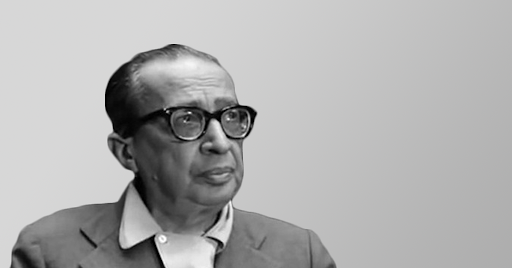
\includegraphics[width=.8\textwidth]{./images/PNLD0010-22}

\vspace{5mm}

\textbf{Poema de uma Quarta-feira de Cinzas}
\thispagestyle{empty}

\begin{verse}
Entre a turba grosseira e fútil
Um Pierrot doloroso passa.
Veste-o uma túnica inconsútil
Feita de sonho e desgraça...

O seu delírio manso agrupa
Atrás dele os maus e os basbaques.
Este o indigita, este outro o apupa...
Indiferente a tais ataques,

Nublada a vista em pranto inútil,
Dolorosamente ele passa.
Veste-o uma túnica inconsútil,
Feita de sonho e desgraça... 
\end{verse}

\bigskip \hfill Manuel Bandeira, 1924

\pagebreak

Por fim, caso sinta que seus alunos estão dispostos a se aprofundar, 
sugira a leitura do artigo \href{}{<<Um Baudelaire para o século XXI>>}, 
escrito pelo poeta e escritor Claudio Cruz, e disponível na 
revista online Sibila. \href{http://sibila.com.br/novos-e-criticos/um-baudelaire-para-o-seculo-xxi/3579}{Clique aqui} para acessar. 
Ou discuta com eles apenas esse trecho do artigo:

\begin{quote}
A lírica moderna, ao contrário, parece ter encontrado em Baudelaire 
o seu inequívoco momento fundador. Talvez (...)
essa unanimidade em torno do chamado ``pai da poesia moderna'' advenha simplesmente 
de ter sido ele o criador do próprio termo modernidade. Seja como for, 
tem-se cada vez mais a impressão de que o ano de 1857, efetivamente, aparece como 
um ano maravilhoso da poesia francesa moderna e, por consequência, ocidental, já que 
é na França que se estabelecem as bases da poesia moderna.
\end{quote}

\subsection{Leitura}

Um dos heróis de Baudelaire, Edgar Allan Poe, usou como epígrafe um verso de 
um escritor francês que traduzia uma experiência tipicamente moderna, ``essa 
grande infelicidade, a de não poder estar só''.
 
``Povoar sua solidão'' e ``estar só em meio a uma massa atarefada'',  
esses dois movimentos se sucedem por todo o livro de Baudelaire, às vezes misturados:
o solitário irrompe na multidão.

Durante a leitura conjunta do livro com seus alunos, 
o que pode tomar alguns dias, proponha uma atividade de escrita criativa 
fora da escola. Escolha uma praça, um museu ou até mesmo café. De lá, peça para os 
alunos descreverem a cena em prosa poética. Diga para não se preocuparem com a qualidade
da escrita, mas apenas com o fluxo da cena, como se fossem pintores. Sugira que colham 
o aspecto das pessoas, trechos de conversa, intensidades do sol, personagens típicos.
A ideia é que o leitor imagine um ``banho de multidão'' e contraste essa experiência 
com a que Baudelaire menciona no poema citado, na <<introdução>> desse manual. 
\BNCC{EM13LGG103} %Escrita criativa

\Image{Félix Nadar (1920-1910), notável fotógrafo francês. Foi também 
jornalista e escritor.}{PNLD0010-20}

Adotando perfis de caminhantes urbanos, sobretudo do \textit{flâneur}, os
estudantes podem percorrer ruas da cidade.

Os alunos também podem descrever a mesma experiência por meio do desenho, 
da música e da fotografia, ou simplesmente gravando em áudio as 
suas impressões. É conveniente portanto que façam uso
de recursos digitais para mapear criativamente o percurso e
experimentar as vivências de urbanas.

\subsection{Pós"-leitura}

Uma das formas mais comuns de contato com a poesia que os jovens 
têm experimentado, principalmente das periferias urbanas, são 
os saraus. Mas o que um sarau de poesia na periferia de um 
país como o Brasil teria em comum com Baudelaire? 

A partir do ensaio da doutora em literatura, Lucia Tennina, 
\href{http://www.scielo.br/pdf/elbc/n42/01.pdf}{<<Saraus das periferias de São Paulo:
poesia entre tragos, silêncios e aplausos>>} publicado na revista 
Estudos de Literatura Brasileira Contemporânea e disponibilizado 
na plataforma SciELO.br, apresente para eles a origem do termo 
\emph{sarau} e algumas hipóteses que justifiquem um encontro de poesia
tão típico das elites estarem sendo agora praticados como forma 
de protesto. Lembre-os da Villa Kyrial, em São Paulo, 
onde a língua ``oficial'' era o francês, e discuta se Baudelaire 
estaria mais para os saraus da periferia ou para práticas 
da elite como as da Villa Kyrial. Como diz a pesquisadora, 
\Image{Jantar na Villa Kyrial, Vila Mariana, São Paulo.}{PNLD0010-21}

\begin{quote}
Os saraus constituíam um microcosmo social que evidenciava uma
sociedade em formação, caracterizada pelo reposicionamento dos indivíduos 
que vivenciavam a passagem de um passado agrícola e patriarcal
para um mundo urbano de ofícios diferenciados, sustentado por novas
alianças e disputas de poder.

No começo do século \textsc{xxi}, essa prática, no momento já deslocada pela
cultura letrada, é retomada e ressignificada manifestadamente nas regiões
periféricas da cidade de São Paulo. Porém, como todo deslocamento de
um domínio de origem para outro, não se tratava de uma cópia dos saraus
das salas das elegantes casas das elites paulistas, mas de múltiplos 
processos que os tornaram diferentes a ponto de não permitir comparações entre
si. Trata"-se, pode"-se dizer, de uma apropriação livre que mantém apenas o
rótulo sarau e a arte como palavra de ordem central.
Os saraus das periferias podem ser definidos, de um modo breve,
como reuniões em bares de diferentes bairros suburbanos da cidade de
São Paulo, onde os moradores declamam ou leem textos próprios ou de outros 
diante de um microfone, durante aproximadamente duas horas. 
\end{quote}

Após essa digressão sobre os saraus urbanos das periferias, proponha
a criação de um sarau chamado ``O brinquedo do pobre'', que tenha como tema um texto de Baudelaire,
que reproduzimos aqui abaixo.
\BNCC{EM13LP47} %Sarau

Este é um 
dos mais célebres poemas em prosa e trata da diferença, ou melhor, da 
falta de diferenças entre
uma criança miserável e uma criança abastada.

\begin{quote}
\textbf{O brinquedo do pobre}\medskip

(...)

Numa estrada, atrás do portão gradeado de um vasto jardim, ao fundo do qual aparecia
a brancura de um belo castelo fustigado pelo sol, estava uma
criança bonita e viçosa, trajando essas roupas campestres de tanta
faceirice.

O luxo, a despreocupação e a visão habitual da riqueza tornam essas
crianças tão bonitas que parecem ter sido moldadas numa massa distinta da
dos filhos da mediocridade ou da pobreza.

A seu lado, jazia na relva um brinquedo maravilhoso, tão viçoso
quanto o dono, envernizado, dourado, vestindo uma roupa púrpura
e coberto de plumas e miçangas. Mas a criança não dava atenção ao seu
brinquedo preferido, e eis o que ela olhava:

Do outro lado da cerca, na estrada, entre os cardos e as urtigas, estava
outra criança, suja, raquítica, fuliginosa, um desses moleques"-párias
de que um olhar imparcial descobriria a beleza se, assim como o olhar do
entendido intui uma pintura ideal sob um verniz de segeiro,
removesse a pátina repulsiva da miséria.

Através dessas grades simbólicas que apartam dois mundos, a estrada e o
castelo, a criança pobre mostrava à criança rica o seu próprio
brinquedo, que esta examinava avidamente como a um objeto raro e
ignorado. Ora, o tal brinquedo, que o moleque sujinho atiçava,
agitava e chacoalhava numa caixa gradeada, era um rato vivo! Os pais,
por economia decerto, tinham tirado o brinquedo da própria vida.

E as duas crianças riam fraternalmente uma para a outra, com dentes de
\textit{igual} brancura.
\end{quote}

\section{Propostas de Atividades II}

\subsection{Pré"-leitura}

Na pré"-leitura, professores da área de Ciências Humanas
podem propor um seminário ou aula conjunta sobre o contexto histórico no qual se insere
a obra de Baudelaire, com ênfase na cidade de Paris, principal cenário que impulsiona a criação artística do autor. 
O objetivo da atividade é mostrar aos estudantes que os temas e personagens da obra de Baudelaire são constituídos no interior da reflexão do artista sobre transformações concretas que edificaram a vida moderna, cujo dinamismo característico desperta a reflexão artística para novos temas, como a efemiridade, o tédio, a melancolia. A contextualização histórica contribui, nesse sentido, para evidenciar as relações entre os aspectos formais e temáticos da obra com as novas experiências vividas cotidianamente pelas pessoas do tempo de Baudelaire.
\BNCC{EM13LP01} %Contexto (História)

Não por acaso, Paris é o principal cenário dos poemas em prosa de Baudelaire. A cidade tornou"-se o centro das convulsões sociais oriundas do processo contraditório de formação da sociedade moderna, o que acarretou, ao longo do século XIX, em crescimento urbano rápido e desordenado, frequentemente interrompido pela irrupção de movimentos populares revolucionários que questionavam a desigualdade social produzida pelo dinamismo moderno. O próprio Baudelaire participa, pessoalmente, de algumas dessas revoluções.

\Image{O novo traçado das cidades atravessou por completo o plano original 
da capital francesa reestruturando a cidade interligada por parques e jardins.}{PNLD0010-24}

Com auxílio do professor de História, realize uma atividade para aproximar os estudantes do contexto histórico de Paris no século \textsc{xix}. Para isso, sugere"-se a divisão da sala em quatro grupos, de modo que cada grupo se responsabilize por uma breve pesquisa sobre as revoluções de 1789, 1830, 1848 e 1871, todas ocorridas em Paris. A pesquisa deve ter como foco os principais valores defendidos em cada um dos processos, suas principais bandeiras e pautas. Seguindo a ordem da temporalidade histórica de cada evento revolucionário, cada grupo deverá realizar uma breve apresentação dos resultados obtidos para o restante da classe. Após as quatro apresentações, proponha uma discussão em sala de aula acerca do caráter conflituoso que marca o processo de formação da sociedade moderna. Tal caráter conflituoso será importante para demarcar, durante a leitura da obra, o seu impacto na ambivalência do texto de Baudelaire, que retrata criticamente os elementos da vida urbana moderna. Abaixo, elenca"-se algumas questões para orientar o debate:

\begin{enumerate}
\item Qual o papel de cada processo revolucionário no longo processo histórico de formação da modernidade?

\item Considerando as quatro revoluções estudadas, pode-se dizer que a formação da sociedade moderna é um processo linear e progressivo? Por quê?

``Quais pautas dos processos estudados se mantêm atuais até os dias de hoje? Por quê?''

\item O que os quatro processos estudados ensinam sobre a vida moderna?
\end{enumerate}

\SideImage{Barão de Haussmann, urbanista responsável pela reconstrução da Paris moderna}{PNLD0010-25}

Após a realização do debate, proponha uma segunda atividade, voltada para demarcar a vida nas cidades (tema caro à Baudelaire) como traço distintivo da sociedade moderna constituída após a Revolução Francesa de 1789. Com auxílio do professor de História, faça uma primeira exposição das principais diferenças entre a sociedade moderna e a sociedade feudal, salientando a importância do surgimento das cidades para o advento da modernidade. Em seguida, proponha um debate entre os alunos sobre as vantagens e desvantagens da vida nas cidades.

% \Image{As avenidas e bulevares de Paris foram uma novidade do novo plano urbanístico para a cidade, mas também uma forma de controlar o fluxo das manifestaões e impedir barricadas.}{PNLD0010-23}



\subsection{Leitura}

Durante a leitura, é possível contextualizar historicamente
os sentimentos de tédio e de melancolia, assim como as figuras do dândi
e do \textit{flâneur}, tipos humanos recorrentes na literatura europeia do
século \textsc{xix}, frequentemente associados à vida nas cidades. Com o auxílio do professor de Geografia, proponha atividades que apontem para a relação entre os temas e personagens de Baudelaire e a dinâmica movimentada das grandes cidades. 
\BNCC{EM13CHS101} %Compreensão de ideias filosóficas




Como primeira atividade, sugere-se a elaboração de discussão acerca das reformas urbanas promovidas em Paris pelo Barão de Haussmann (1808--1891)
(em francês, pronuncia-se /osmã/) e os impactos que as transformações da geografia urbana de Paris geram no cotidiano dos habitantes das cidades. Para isso, convém dividir a turma em duplas ou trios (a depender do tamanho da sala) e munir cada dupla ou trio com dois grupos diferentes de imagens: o primeiro grupo de imagens retratando Paris antes da reforma de Haussman; o segundo grupo de imagens retratando Paris após a reforma de Haussman. Após alguns minutos para a discussão entre os grupos, cada um deverá apresentar para a classe um elemento que observou sobre as diferenças os dois momentos da cidade de Paris, antes e depois da reforma. Os grupos não podem repetir os elementos já destacados pelos grupos anteriores. Uma vez listado os principais elementos destacados por cada grupo, proponha a leitura coletiva do seguinte trecho da obra de Baudelaire:

\begin{quote}
\dotfill

\textbf{\textsc{xxiv.} Os projetos}\medskip

Ele pensava, enquanto passeava num grande parque deserto:
``Que linda ela ficaria com um traje de corte, complicado
e fastuoso, descendo, na atmosfera de um belo entardecer, os
degraus de mármore de um palácio, diante dos grandes gramados e açudes!
Pois ela tem naturalmente um ar de princesa!''

Passando mais tarde numa rua, parou em frente a uma loja de gravuras
e, ao encontrar numa pasta uma estampa representando uma paisagem
tropical, pensou: ``Não! Não é num palácio que eu gostaria
de possuir sua querida vida. Não estaríamos \textit{em casa}. Aliás, essas
paredes crivadas de ouro não deixariam um só espaço para pendurar sua
imagem; nestas solenes galerias, não há um só recanto para a
intimidade. Realmente, \textit{aqui} é que teria de morar para cultivar
o sonho de minha vida''.

E enquanto analisava os detalhes da gravura, prosseguia mentalmente:
``À beira-mar, uma linda choupana de madeira, envolta
em todas essas árvores estranhas e reluzentes cujos nomes esqueci\ldots\ 
na atmosfera, um cheiro embriagante, indefinível\ldots\  na choupana, um
forte aroma de rosa e almíscar\ldots\  adiante, atrás da nossa
pequena propriedade, pedaços de mastros balançados pelo marulho\ldots\  à nossa volta, para além do quarto aclarado por uma luz rosada filtrada
pelos estores, decorada com esteiras novas e flores capitosas, raras poltronas de um rococó português, de madeira pesada e escura (em
que ela repousaria tão calma, tão arejada, tragando o fumo
levemente opiáceo!), para além da varanda, o tumulto dos pássaros bêbados de
luz e o tagarelar das negrinhas\ldots\  e à noite, para servir de
acompanhamento aos meus sonhos, o canto sentido das árvores musicais,
as melancólicas casuarinas! Sim, na verdade, é este o cenário que eu
buscava. Para que iria querer palácios?''

Mais adiante, ao percorrer uma larga avenida, avistou uma pousada
asseadinha onde, a uma janela enfeitada com cortinas de chita
estampada, se debruçavam dois rostos risonhos. E, logo:
``Meu pensamento'' --- refletiu --- ``deve ser muito vagamundo
para ir buscar tão longe o que está tão perto de mim. O prazer e a
felicidade estão na primeira pousada que aparece, na pousada do
acaso, tão fecunda em volúpias. Um bom fogo, faianças vistosas, um
jantar passável, um vinho rude e uma cama bem ampla com lençóis um
pouco ásperos, mas limpos; haverá coisa melhor?''

E ao voltar sozinho para casa, nesta hora em que os conselhos da
Sabedoria já não são sufocados pelo burburinho da vida exterior,
ele pensou: ``Tive hoje, em sonhos, três domicílios em que
encontrei igual prazer. Por que obrigar meu corpo a mudar de lugar, 
se minha alma é tão ligeira em viajar? E de que serve executar projetos,
se o projeto, em si, já é fruição suficiente?''

\dotfill
\end{quote}

Após a leitura, promova um debate em sala de aula, norteado pelas seguintes questões:

\begin{enumerate}
\item Qual o papel da geografia urbana de Paris nas reflexões da personagem?
\item Qual a relação entre a vida movimentada da cidade e os diferentes sonhos da personagem que passea pelas ruas e parques?
\item Quais traços da reforma urbana de Haussmann se fazem visíveis (ou não) no texto?
\item O que quer dizer o narrador quando perguna: 'de que serve executar projetos, se o projeto, em si, já é fruição suficiente?
\item Qual a crítica da vida moderna se pode extrair dessa última frase?
\end{enumerate}

\Image{Charles Baudelaire em 1863. (Etienne Carjat; CC-BY 2.0)}{PNLD0010-03.png}

``Quais traços da reforma urbana de Haussmann se fazem visíveis (ou não) no texto?''

``O que quer dizer o narrador quando pergunta: 'de que serve executar projetos, se o projeto, em si, já é fruição suficiente?' Qual a crítica da vida moderna se pode extrair dessa última frase?''

\subsection{Pós"-leitura}

Neste último momento, sugerimos diálogos, em conjunto com
professores de Ciências Humanas, sobretudo com o professor de História, acerca da importância da obra de Baudelaire para refletir sobre
a natureza da sociedade moderna constituída nos séculos \textsc{xviii} e \textsc{xix}. O objetivo da atividade é salientar a ambivalência que caracteriza a poética de Baudelaire, que quer ser o poeta de seu tempo e, nesse sentido, retrada a realidade moderna criticamente a partir de seu principal cenário, a cidade, e seu novo sujeito, as multidões. Como inventor do termo \textit{modernidade}, Baudelaire é um dos principais autores do século \textsc{xix}, e percebeu a intensidade dos efeitos das mudanças sociais e econômicas de seu tempo.
\BNCC{EM13LP52} %Estrutura de texto (Cânone)

Retome em sala de aula a leitura do seguinte trecho do livro:

\begin{quote}
\dotfill

\textbf{\textsc{xii.} As massas}\medskip

Não é dado a qualquer um tomar banho de multidão. Desfrutar da massa é uma
arte e só poderá fazer, às custas do gênero humano, uma orgia de
vitalidade, aquele a quem uma fada terá insuflado no berço o gosto
pelo disfarce e a máscara, o ódio do domicílio e a paixão pela
viagem.

Multidão, solidão: termos iguais e permutáveis, para o poeta ativo e
fecundo. Quem não sabe povoar sua solidão tampouco sabe estar só em
meio a uma massa azafamada.

Goza o poeta desse incomparável privilégio de poder ser, a bel-prazer,
ele próprio e outrem. Igual a essas almas errantes em busca de um corpo,
ele entra, quando quer, na personagem de qualquer um. Para ele apenas, tudo
está vacante; e se alguns lugares lhe parecem estar fechados, é que a
seus olhos não valem a pena ser visitados.

O andarilho solitário e pensativo tira uma embriaguez singular desta
universal comunhão. Quem desposa facilmente a massa conhece gozos
febris, dos quais serão eternamente privados o egoísta, trancado como
um cofre, e o preguiçoso, internado como um molusco. Ele adota como
suas todas as profissões, todas as alegrias e todas as misérias que a
circunstância lhe apresenta.

O que os homens denominam amor é bem pequeno, restrito e frágil, se 
comparado a esta inefável orgia, a esta santa prostituição da alma
que se dá por inteiro, poesia e caridade, ao imprevisto que se mostra, ao
desconhecido que passa.

É bom ensinar, às vezes, aos venturosos deste mundo, mesmo que só para
humilhar por um instante seu orgulho tolo, que existem venturas
superiores às suas, mais amplas e refinadas. Os fundadores de colônias,
os pastores de povos, os padres missionários exilados no fim do mundo,
decerto conhecem algo destas misteriosas embriaguezes; e, no seio da
vasta família que seu gênio construiu para si, eles por vezes devem rir
dos que se compadecem com sua sina tão agitada e sua vida tão
casta.

\dotfill
\end{quote}

Com o auxílio do professores de \textbf{História} e \textbf{Geografia}, divida a turma em grupos e proponha a realização de um debate em torno das seguintes questões:

\begin{enumerate}
\item O autor apresenta uma visão positiva da vida na cidade?
\item Na sua opinião, por quê o autor associa a multidão da cidade ao sentimento de solidão?
\end{enumerate}

Após a realização dos debates internos, cada grupo deverá, num segundo momento, apresentar a síntese de suas reflexões para toda a sala. Ao final da atividade, cada aluno poderá redigir um texto dissertativo respondendo a seguinte questão:

\begin{itemize}
\item Com base na leitura da obra, Baudelaire pode ser considerado um crítico da vida moderna? Por quê?
\end{itemize}

\section{Aprofundamento}

Nesta seção, desenvolvemos um trabalho de aprofundamento que, em diálogo
com a formação continuada de professores, oferece subsídios para a
abordagem do texto literário.

Charles Baudelaire, escritor francês, é ainda hoje reverenciado como
um dos paradigmas máximos da criação poética.
Dono de uma imagética original, Baudelaire foi também um influente
crítico de arte e um tradutor de grande envergadura.

De alma inquieta e conturbada, Baudelaire via com desconfiança a era do
progresso, mesmo sendo o precursor da poesia lírica moderna.
Ele via na modernidade uma morbidez oculta que sua sensibilidade não
tolerava.


\Image{Retrato de Baudelaire pintado por Émile Deroy, em 1844. (Émile Deroy; CC-BY-SA-4.0)}{PNLD0010-05.png}
 

Em 1857, publicou \textit{As flores do mal},
sua obra"-prima, na qual ofende a moral burguesa. Acabou sofrendo um
processo em que foi obrigado a pagar uma multa considerável, além de
suprimir sete poemas do livro.

A obra é tão importante quanto \textit{As flores do mal} na obra de
Baudelaire e está entre as obras de poesia mais importantes da
literatura universal.
Baudelaire ataca convenções e é um verdadeiro artesão da palavra.


%\Image{Desenho de Baudelaire feito pelo artista Édouard Manet (Édouard Manet; Domínio Público)}{PNLD0010-06.png}


Mal compreendida por seus contemporâneos, a poesia de Baudelaire está
marcada pela contradição. de um lado, revela o romantismo de Allan Poe e
Gérard de Nerval, e de outro, o poeta crítico que se opôs aos excessos
sentimentais e retóricos do romantismo francês.

Baudelaire afirmava que a finalidade de sua poesia era ``extrair a
beleza do mal'' e comunicar aos homens a tragédia essencial do ser
humano, dividido entre deus e o demônio.
Segundo o crítico alemão Erich Auerbach, o poeta criou a poesia moderna
ao incorporar à literatura a realidade grotesca. O escritor André Breton
considerava Baudelaire o primeiro dos surrealistas.

O livro de Baudelaire perfaz um todo, apesar da aparente dispersão dos
contos.
O conto, gênero breve cuja ação tende diretamente ao final, com uma
unidade dramática, foi admirado por Baudelaire e Edgar Allan Poe.

Já nos poemas, Baudelaire explora recursos de imagem e sonoridade que
evocam o onírico e o fantástico, para além da realidade cotidiana.
Mas o que é o poema em prosa, que praticamente se autonomizou como um
gênero?.

A ``prosa poética'' utiliza um grupo de recursos mais comuns na poesia,
como aliterações, ecos (rimas), um ritmo demarcado mais claramente.
Só que os ``pequenos poemas em prosa'' são antes de mais nada poemas,
escritos utilizando aquela outra forma, a prosa, como veículo.

Baudelaire será seguido nessa forma dos poemas em prosa por dois dos
mais importantes poetas franceses do fim do século: Mallarmé e
Rimbaud.
Além deles, todos os decadentistas e simbolistas derivam muita coisa
das descobertas e da sensibilidade de Baudelaire, assim como o
modernismo internacional.

\Image{O escritor Edgar Allan Poe, grande inspiração de Baudelaire. (Autor desconhecido, fotografia restaurada por Yann Forget e Adam Cuerden ; Domínio Público)}{PNLD0010-08.png}


Além de ser evidentemente, um precursor de todos os grandes poetas
simbolistas, Baudelaire é considerado pela maior parte dos críticos como
marco fundador da poesia moderna. Isso se deve ao fato de que, pela
percepção do real, chegava sempre a um equivalente do
sentimento que desejasse expressar.

Isso acontece, por exemplo, no poema ``correspondências'', de
\emph{As flores do mal}, onde Baudelaire expõe a origem de seu ``projeto simbólico''.
Desta forma, sua poesia tendeu para a expressão de imagens cotidianas, o
``visto pelo autor'', tendo, o poeta, sido quem melhor, em sua época,
intuiu a mudança radical provocada pela
metrópole sobre a
sensibilidade, tratando de tipos sociais urbanos, como o \textit{flaneur} --
caminhante das galerias de grandes cidades -- e o dandi -- o excentrico
admirador de obras de arte e cultivador de luxos e hábitos excêntricos.


\Image{Estátua "O Flaneur": um tipo social retratado pelo autor, que representa o caminhante de galerias de grandes cidades. (PVT Pauline; CC-BY-SA 3.0)}{PNLD0010-07.png}


É uma ideia até certo ponto bizarra dizer que esse quase misantropo
fosse um ``homem das multidões'', mas a imersão na massa das cidades
grandes está presente em sua experiência poética.
Quem ressaltou esse aspecto de sua obra foi o pensador Walter Benjamin,
na obra \textit{Charles Baudelaire: um lírico no auge do capitalismo}, em
que descreve a atmosfera de Paris a partir da figura do \textit{flaneur}, um
tipo de caminhante urbano que surge com a modernização das cidades e o
apogeu das galerias, cafés e boulevares parisienses.


\Image{"Carnaval parisiense": a sensação de estar imerso na multidão na cidade é um dos assuntos tratados pelo autor.  (Anônimo; CC-BY-SA 3.0)}{PNLD0010-10.png}


O leitor moderno precisa fazer um exercício de imaginação para apreender
o que terá sido alguém desvinculado da preocupação imediata com as
coisas cotidianas e materiais.
O dândi do século \textsc{xix} é um personagem excêntrico e um crédito
ilimitado poderia lhe bastar para viver luxuosamente e distante dos
mortais, como um aristocrata.

Baudelaire tinha o sentido desse primado absoluto da estética, do
desejo da perfeição na beleza e no horror, mas sabia também que ``o
estudo do belo é um duelo em que o artista grita de pavor antes de ser
vencido''.
Ao esteta e ao dândi, na figura de Baudelaire, junta"-se o \textit{flaneur},
que é aquele que flana, ou vive a deambular, caminhar sem rumo pela
cidade.

Isso é importante:. o \textit{flâneur} não está indo a lugar algum, ele está de
passagem, e isso se reflete no modo como esses textos devem ser lidos,
pois eles resvalam na ideia da cidade, que figura inúmeras sugestões ao observador atento.
Baudelaire ainda dinamiza aquela incrível e insuspeita força moral sobre
seus objetos de atenção.
São cenas passageiras, na rua ou dentro de um teatro da imaginação, e
ao mesmo tempo exibem eternidade, numa analogia com a recém"-surgida
fotografia, que nascia com o objetivo de recortar e congelar o
momento.

Já ``spleen'' é uma palavra que designa um ``tédio existencial''.
Podemos definir o spleen como uma espécie de melancolia pensante.
Ele se aplica, como vemos, diretamente à vida nas então recentes
metrópoles e, em particular, em Paris.


\Image{A atmosfera de Paris é retratada pelo autor, especialmente no tema da solidão. (Stockholm Transport Museum; Domínio Público)}{PNLD0010-09.png}


E Paris, no livro de Baudelaire, é mais que uma cidade. É um estado
mental e um espaço personificado.
\emph{Pequenos poemas em prosa} ou \emph{O spleen de paris}, obra póstuma,
publicada em 1869, consumiu mais de dez anos até sua forma definitiva.
Muitos dos poemas já haviam aparecido em jornais e receberam de pronto a
admiração da crítica e do público.

\section{Sugestões de referências complementares}\label{sugestoes}

% Ainda a construir.
\subsection{Filmes}

\textit{O convite à viagem}. Direção: Germaine Dulac. (França, 1927).

Baseado no poema homônimo de Baudelaire, é um filme mudo do começo do século \textsc{xx}
que nos permite ter alguma ideia do cenário urbano sobre o qual o poeta fala em seus poemas.
O filme está disponível gratuitamente e legendado no seguinte acesso: \href{https://www.youtube.com/watch?v=wCZgaPcs6Y0}{``L'invitation au voyage''.}

\textit{A Serpente que dança}. Direção: João de Mendonça Lima Filho. (Brasil, 2013).

Inspirado no poema homônimo, localizado no livro \textit{As flores do mal}, é um curta"-metragem
de 7 minutos de duração que investiga a transposição da poética de Baudelaire para a imagem em movimento.

\textit{Paraísos Artificiais}. Direção: Marcos Prado. (Brasil, 2012).

Inspirado no livro homônimo de Baudelaire, o filme discute a questão das drogas na sociedade,
sobretudo entre os jovens, que, no filme, acham nela um propulsor de experiências intensas.

\subsection{Museus}

No Museu Nacional de Belas Artes, no Rio de Janeiro, se encontra um retrato de Charles 
Baudelaire feito pelo pintor impressionista Édouard Manet. A obra pode ser acessada
pelo \emph{Google Arts and Culture}: \href{https://artsandculture.google.com/asset/retrato-de-charles-baudelaire-%C3%89douard-manet/yAFFnToINzBuUg?hl=pt-br}{Museu Nacional de Belas Artes}: Retrato de Charles Baudelaire, 1865.

%https://revistacaliban.net/charles-baudelaire-o-esgrimista-da-modernidade-4a22a92e4d00

\section{Bibliografia comentada}

\begin{itemize}
\item\textsc{baudelaire}, Charles. \textit{As flores do mal}. São Paulo:
Penguin"-Companhia das Letras, 2019.

Este volume bilíngue reúne toda a poesia de Baudelaire: \textit{As flores do mal}
tal como publicado em 1861 e os poemas acrescidos à edição póstuma de
1868.

\item\textsc{benjamin}, Walter. \textit{Charles Baudelaire: um lírico no auge do
capitalismo}. São Paulo: Brasiliense, 1989.

Ao decifrar os nexos entre a obra de Baudelaire e as relações sociais
que se afirmavam na Europa Ocidental do final do século passado Benjamin
inova com relação à crítica literária e à análise sociológica
tradicionais.

\item\textsc{bosi}, Alfredo. \textit{O ser e o tempo da poesia}. São Paulo: Companhia
das Letras, 2000.

São ensaios no sentido mais nobre do gênero: jogo criativo da
inteligência a mover"-se, alerta e sensível, no espaço que vai do geral
ao particular; dos parâmetros da essência às formas de sua atualização
histórica; do ser ao tempo da poesia.

\item\textsc{friedrich}, Hugo. \textit{Estrutura da lírica moderna}. São Paulo: Duas
Cidades, 1978.

A anormalidade da lírica moderna diz respeito às composições deslocadas
da realidade e autônomas em seus significados, ou seja, a anormalidade
da lírica moderna prescreve seus efeitos na união do irreal com
elementos logicamente limitados.

\item\textsc{teles}, Gilberto Mendonça. \textit{Vanguarda europeia e modernismo
brasileiro}. Rio de Janeiro: José Olympio, 2012.

Vanguarda europeia \& modernismo brasileiro reúne poemas, manifestos e
conferências vanguardistas publicados entre 1857 e 1972, reunindo tais
textos numa única fonte de consulta.


\item\textsc{novaes}, Adauto. \textit{Poetas que pensaram o mundo}. São Paulo:
Companhia das Letras, 2005.

Os poetas"-filósofos que participam desta coletânea tratam não apenas de
poesia, mas da história do pensamento através da poesia. Diante dos
múltiplos caminhos que percorrem este livro, o leitor começa por onde
quiser.

\item\textsc{starobinski}, Jean. \textit{A melancolia diante do espelho: três leituras de Baudelaire}. São Paulo: Editora 34, 2014.

A melancolia diante do espelho examina com sensibilidade e minúcia três
poemas das Flores do Mal, de Charles Baudelaire. O foco do autor são os
caminhos pelos quais Baudelaire renova o tema da melancolia na arte
ocidental.

\item\textsc{troyat}, Henri. \textit{Baudelaire}. São Paulo: Editora Pagina Aberta Ltda Scritta, 1995.

A obra de Henri Troyat relata a biografia do famoso poeta francês
Charles Baudelaire, contextualizando sua obra e seu tempo.
\end{itemize}


\end{document}